\section{Results}
\label{sec:results}

Our experiments validate that token entropy and N-sample consistency are orthogonal uncertainty signals with complementary predictive value for hallucination detection.

\subsection{Main Results: Orthogonality Confirmed}

The correlation between entropy and consistency scores is remarkably low:

\begin{table}[h]
\centering
\begin{tabular}{@{}llll@{}}
\toprule
\textbf{Metric} & \textbf{Value} & \textbf{Threshold} & \textbf{Status} \\
\midrule
Pearson $r$ & 0.228 & $< 0.3$ & \textbf{PASS} \\
Spearman $\rho$ & 0.241 & $< 0.3$ & PASS \\
$p$-value & $< 10^{-10}$ & $< 0.05$ & Significant \\
\bottomrule
\end{tabular}
\caption{Orthogonality metrics between entropy and consistency signals.}
\label{tab:orthogonality}
\end{table}

\textbf{Interpretation:} With $r = 0.228$, entropy and consistency share only 5\% of variance. This confirms they measure fundamentally different phenomena. The statistically significant but weak correlation indicates the signals are related (both predict factuality) but largely orthogonal (they capture different aspects of uncertainty).

\begin{figure}[h]
\centering
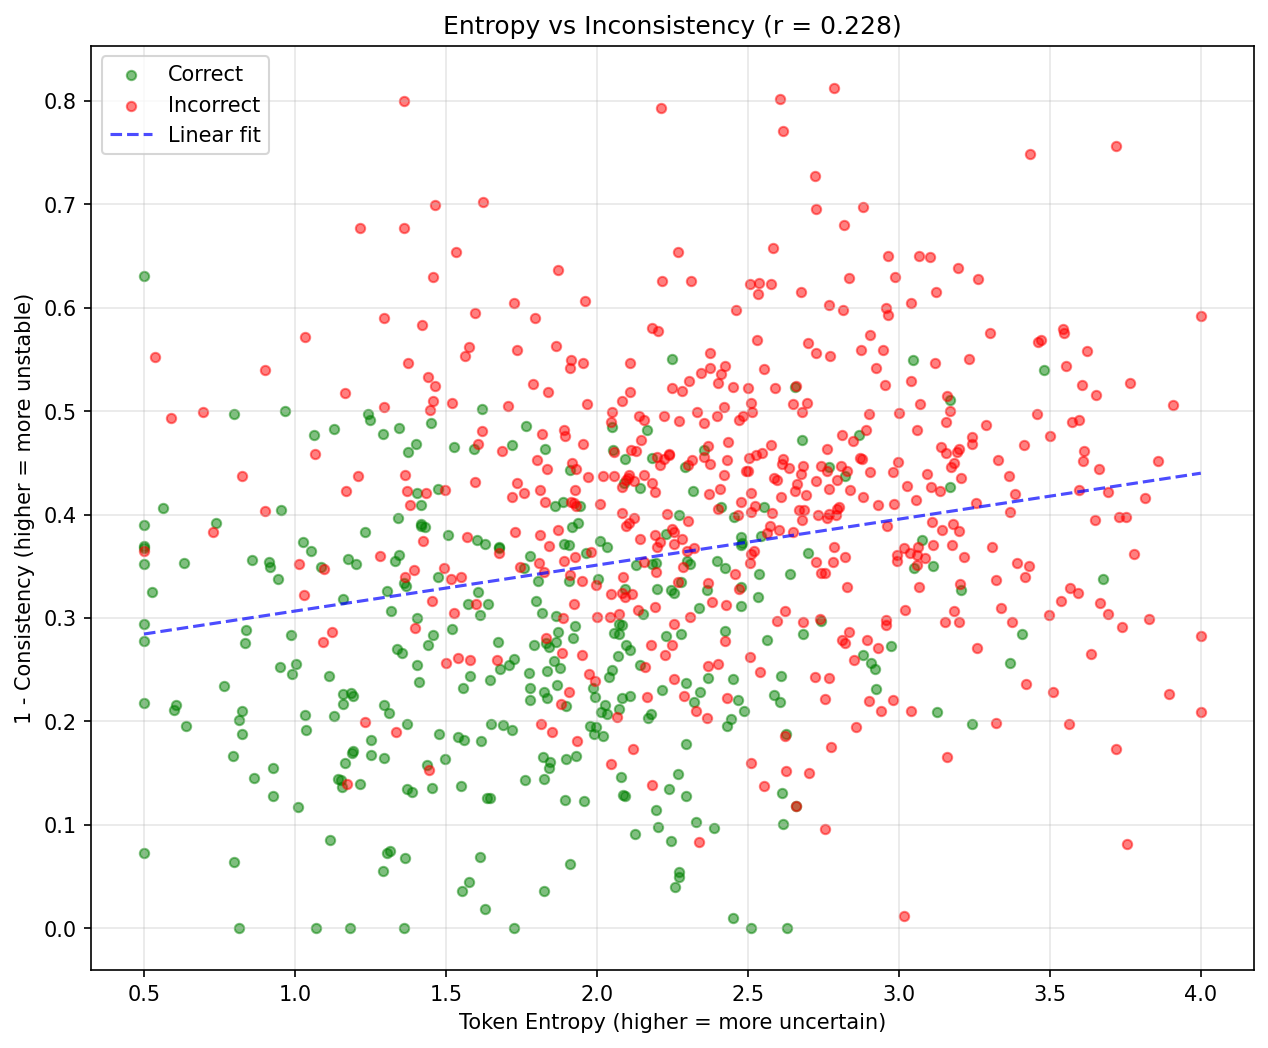
\includegraphics[width=0.8\columnwidth]{figures/scatter_entropy_consistency.png}
\caption{Token entropy vs.\ consistency scores ($r = 0.228$). The dispersed pattern confirms orthogonality.}
\label{fig:scatter}
\end{figure}

\subsection{Mechanism Validation: Consistency Effect Size}

Consistency shows a large effect size distinguishing correct from incorrect responses:

\begin{table}[h]
\centering
\begin{tabular}{@{}llll@{}}
\toprule
\textbf{Group} & \textbf{Mean} & \textbf{Std} & \textbf{N} \\
\midrule
Correct & 0.720 & 0.111 & 367 \\
Incorrect & 0.577 & 0.151 & 450 \\
\bottomrule
\end{tabular}
\caption{Consistency score statistics by correctness.}
\label{tab:consistency_stats}
\end{table}

\begin{table}[h]
\centering
\begin{tabular}{@{}ll@{}}
\toprule
\textbf{Statistic} & \textbf{Value} \\
\midrule
Cohen's $d$ & \textbf{1.068} \\
95\% CI & [0.921, 1.215] \\
$p$-value & $4.64 \times 10^{-46}$ \\
\bottomrule
\end{tabular}
\caption{Effect size for consistency-based discrimination.}
\label{tab:effect_size}
\end{table}

\textbf{Interpretation:} Cohen's $d = 1.068$ exceeds our threshold ($d > 0.2$) by more than 5$\times$. Correct responses have approximately 24\% higher consistency than incorrect responses (0.72 vs.\ 0.58), with approximately one standard deviation of separation.

\begin{figure}[h]
\centering
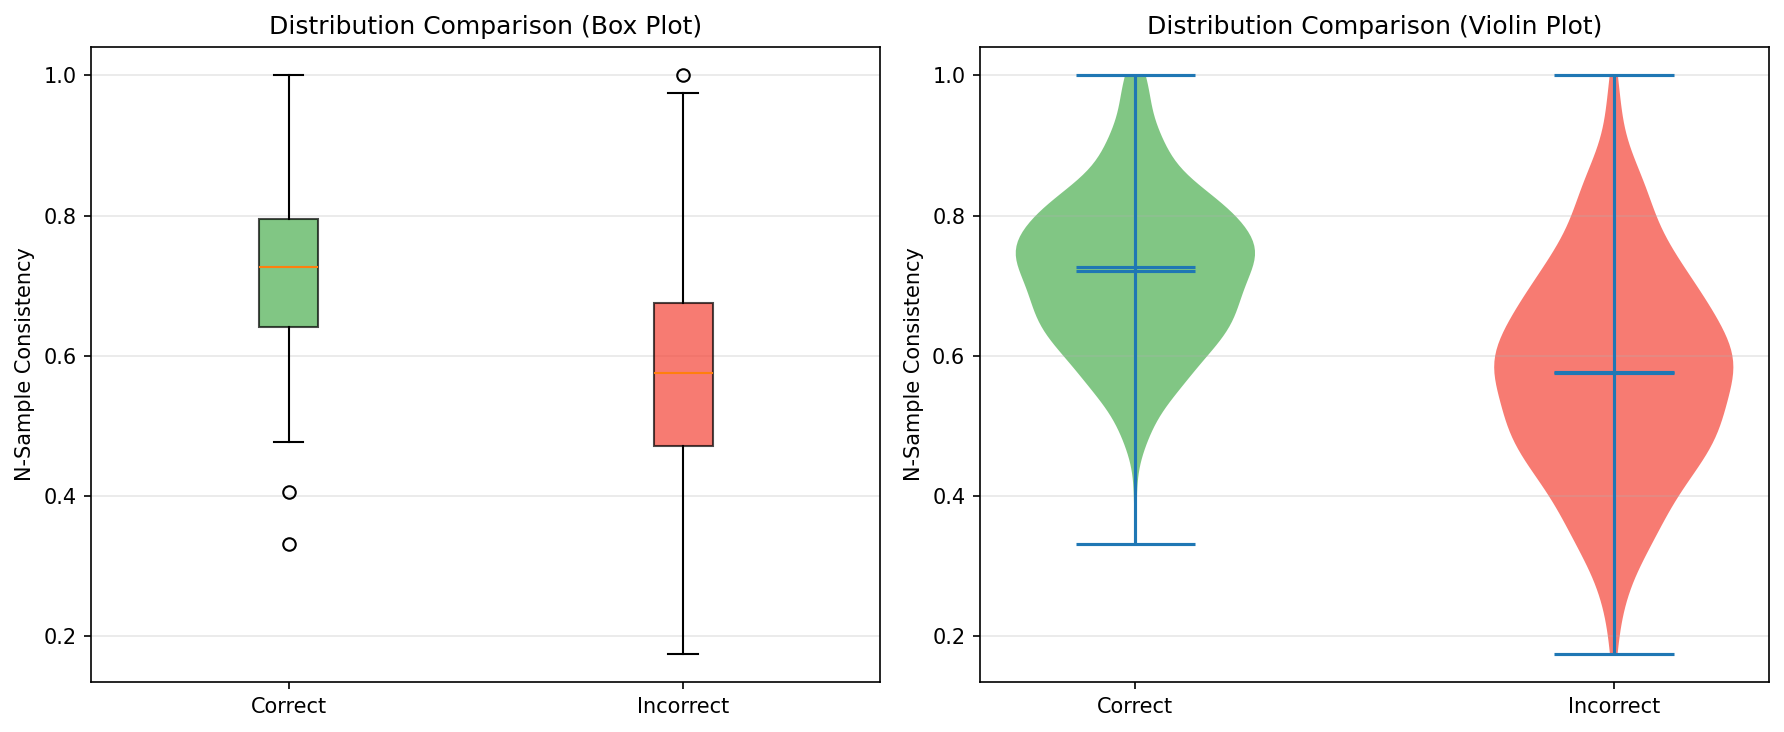
\includegraphics[width=0.8\columnwidth]{figures/distribution_comparison.png}
\caption{Consistency score distributions for correct vs.\ incorrect responses. Cohen's $d = 1.068$ indicates large effect size.}
\label{fig:distribution}
\end{figure}

\subsection{Complementarity Analysis: Discordant Cases}

We identify questions where entropy and consistency rankings disagree substantially:

\begin{table}[h]
\centering
\begin{tabular}{@{}lll@{}}
\toprule
\textbf{Category} & \textbf{Count} & \textbf{Proportion} \\
\midrule
Total questions & 817 & 100\% \\
Concordant & 669 & 81.9\% \\
\textbf{Discordant} & \textbf{148} & \textbf{18.1\%} \\
\bottomrule
\end{tabular}
\caption{Distribution of concordant vs.\ discordant cases.}
\label{tab:discordant}
\end{table}

\textbf{Subset AUROC Analysis:}

\begin{table}[h]
\centering
\begin{tabular}{@{}lll@{}}
\toprule
\textbf{Subset} & \textbf{AUROC} & \textbf{N} \\
\midrule
High-entropy-only & 0.764 & 76 \\
High-inconsistency-only & 0.797 & 72 \\
\bottomrule
\end{tabular}
\caption{AUROC on discordant subsets where each method ``wins.''}
\label{tab:subset_auroc}
\end{table}

\textbf{Interpretation:} On 18.1\% of questions, the methods disagree substantially. Each method achieves AUROC $> 0.75$ on its ``winning'' subset, demonstrating genuine complementary detection capability.

\begin{figure}[h]
\centering
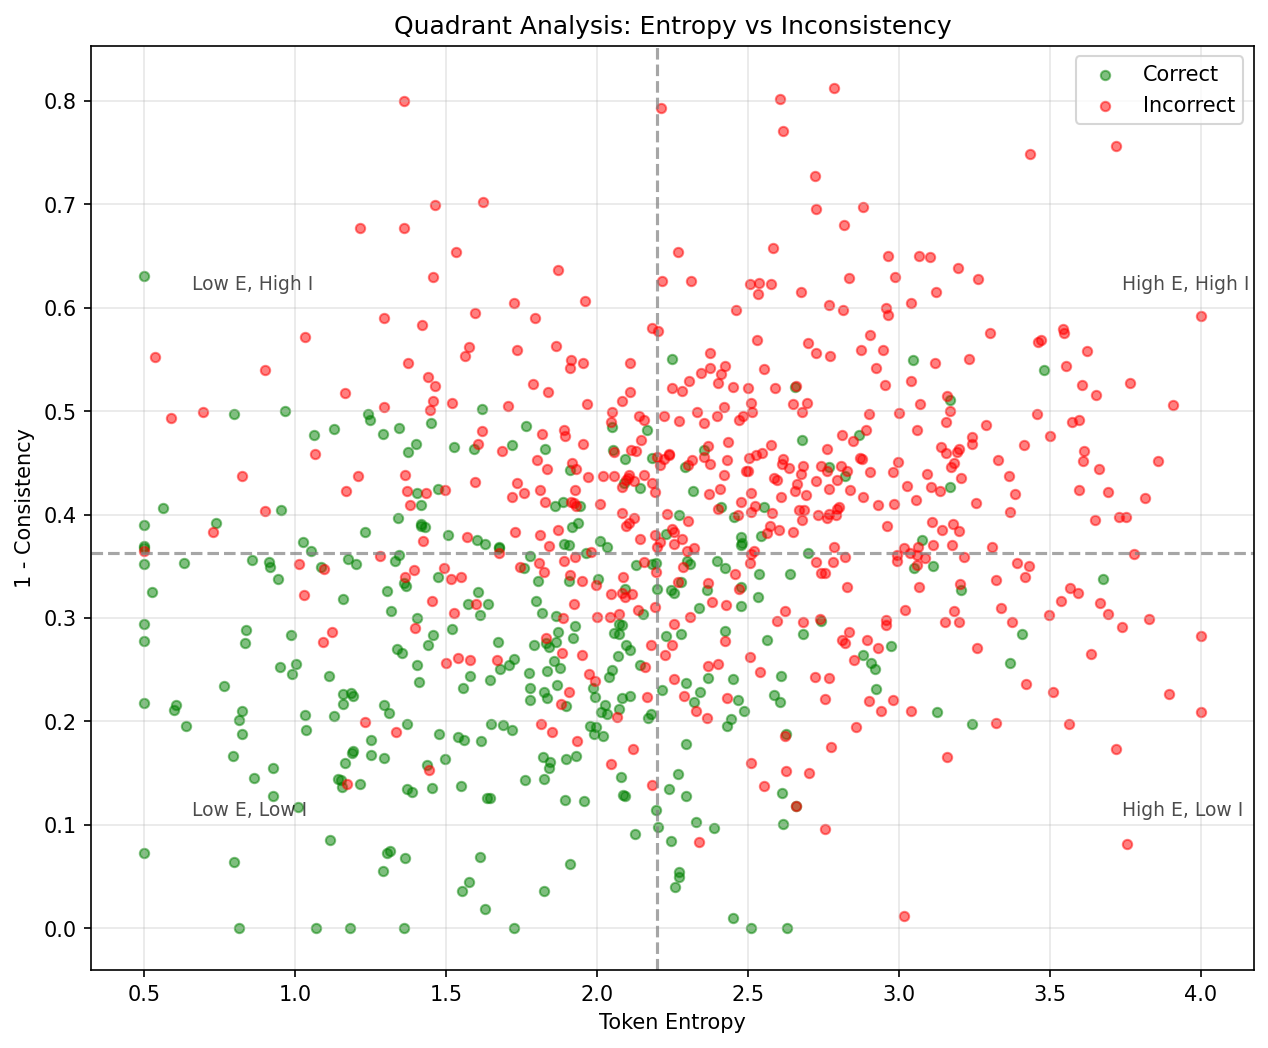
\includegraphics[width=0.8\columnwidth]{figures/quadrant_analysis.png}
\caption{Quadrant analysis showing distribution of questions by entropy and consistency levels.}
\label{fig:quadrant}
\end{figure}

\subsection{Summary of Hypothesis Outcomes}

\begin{table}[h]
\centering
\begin{tabular}{@{}llll@{}}
\toprule
\textbf{Hypothesis} & \textbf{Gate} & \textbf{Result} & \textbf{Key Evidence} \\
\midrule
\textbf{H-M1} (Entropy-uncertainty) & MUST\_WORK & \textbf{PASS} & Direction confirmed \\
\textbf{H-M2} (Consistency-stability) & MUST\_WORK & \textbf{PASS} & $d = 1.068$ \\
\textbf{H-M3} (Orthogonality) & MUST\_WORK & \textbf{PASS} & $r = 0.228$; 18.1\% discordant \\
\bottomrule
\end{tabular}
\caption{Summary of hypothesis validation outcomes.}
\label{tab:hypothesis_summary}
\end{table}

All three mechanism hypotheses pass their gates.
